%
% Exemplo LaTeX de monografia UNISINOS
%
% Elaborado com base nas orientações dadas no documento
% ``GUIA PARA ELABORAÇÃO DE TRABALHOS ACADÊMICOS''
% disponível no site da biblioteca da Unisinos.
% http://www.unisinos.br/biblioteca
%
% Os elementos textuais abaixo são apresentados na ordem em que devem
% aparecer no documento.  Repare que nem todos são obrigatórios - isso
% é devidamente indicado em cada caso.
%
% Comentários abaixo colocados entre aspas (`` '') foram
% extraídos diretamente do documento da biblioteca.
%
% Este documento é de domínio público.
%

%=======================================================================
% Declarações iniciais identificando a classe de documento e
% selecionando alguns pacotes adicionais.
%
% As opções disponíveis (separe-as com vírgulas, sem espaço) são:
% - twoside: Formata o documento para impressão frente-e-verso
%   (o default é somente-frente)
% - english,brazilian,french,german,etc.: idiomas usados no documento.
%   Deve ser colocado por último o idioma principal.
%=======================================================================
\documentclass[twoside,english,brazilian]{UNISINOSmonografia}
\usepackage[utf8]{inputenc} % charset do texto (utf8, latin1, etc.)
\usepackage[T1]{fontenc} % encoding da fonte (afeta a sep. de sílabas)
\usepackage{graphicx} % comandos para gráficos e inclusão de figuras
\usepackage{bibentry} % para inserir refs. bib. no meio do texto

%=======================================================================
% Escolha do sistema para geração de referências bibliográficas.
%
% O default é usar o estilo unisinos.bst.  Comente a definição abaixo
% e descomente a linha seguinte para usar o estilo do ABNTeX (é
% necessário ter esse pacote instalado).
%
% A vantagem do unisinos.bst é que ele permite o uso de um arquivo .bib
% seguindo as orientações tradicionais do BibTeX (veja essas orientações
% em http://ctan.tug.org/tex-archive/biblio/bibtex/contrib/doc/btxdoc.pdf).
% Entretanto, o estilo não suporta algumas citações mais exóticas como
% apud.  Para isso, use o ABNTeX, mas esteja ciente de que muitas de
% suas referências serão incompatíveis com os estilos tradicionais do
% BibTeX como plain, alpha, ieeetr, entre outros.
%=======================================================================
\usepackage[alf]{abntex2cite}
%\usepackage[alf]{abntcite}

%=======================================================================
% Dados gerais sobre o trabalho.
%=======================================================================
\autor{Aguiar Plentz}{Christian}
\titulo{Técnicas de Anti-Aliasing, Super Sampling e o uso de Deep Learning}
\orientador[Professora]{Baptista Queiroz}{Rossana}
%\coorientador[Prof.~Dr.]{Lamport}{Leslie}

\unidade{Unidade Acadêmica de Graduação}
\curso{Curso de Bacharelado em Ciência da Computação}
\natureza{%
Monografia apresentada como requisito parcial para obtenção do título de Bacharel em Ciência da Computação, pelo Curso de Ciência da Computação da Universidade do Vale do Rio dos Sinos (UNISINOS)
}
\local{São Leopoldo}
\ano{2026}

% dados da ficha catalográfica
% (obrigatória somente para dissertações e teses)
%\cip{Dissertação (mestrado)}{004.732}
%\bibliotecario{Bibliotecária responsável: Fulana da Silva}{12/3456}

% cada palavra-chave deve ser fornecida duas vezes, uma em português e
% outra no idioma estrangeiro (na verdade, em tantos idiomas quantos se
% desejar).
\palavrachave{brazilian}{Computação Gráfica}
\palavrachave{brazilian}{Anti-Aliasing}
\palavrachave{brazilian}{Godot}
\palavrachave{brazilian}{Upscaling}
\palavrachave{english}{Computer Graphics}
\palavrachave{english}{Anti-Aliasing}
\palavrachave{english}{Godot}
\palavrachave{english}{Upscaling}

%=======================================================================
% Início do documento.
%=======================================================================
\begin{document}
\capa
\folhaderosto
%\folhadeaprovacao % não deve ser incluída nos TCCs

%=======================================================================
% Dedicatória (opcional).
%
% O texto é normalmente colocado na parte de baixo da página, alinhado
% à direita.  Mas a formatação é basicamente livre.  Só não se escreve
% a palavra 'dedicatória'.
%=======================================================================
% \begin{dedicatoria}
% Aos nossos pais.\\[4ex] % quebra a linha dando um espaçamento maior
% \begin{itshape} % faz o texto ficar em itálico
% If I have seen farther than others,\\
% it is because I stood on the shoulders of giants.\\
% \end{itshape}
% --- \textsc{Sir Isaac Newton} % \textsc é o "small caps"
% \end{dedicatoria}

%=======================================================================
% Agradecimentos (opcional).
%=======================================================================
% \begin{agradecimentos}
% Obrigado!
% \end{agradecimentos}

%=======================================================================
% Epígrafe (opcional).
%
% ``[...] o autor apresenta uma citação, seguida de indicação de autoria,
% relacionada com a matéria tratada no corpo do trabalho. Podem, também,
% constar epígrafes nas folhas de aberturas das seções primárias.''
%=======================================================================
% \begin{epigrafe}
% ``\textit{Ninguém abre um livro sem que aprenda alguma coisa}''.\\
% (Anônimo)
% \end{epigrafe}

%=======================================================================
% Resumo em Português.
%
% A recomendação é para 150 a 500 palavras.
%=======================================================================
\begin{abstract}
Este artigo busca comparar as variadas técnicas de Anti-Aliasing para comparar sua qualidade de imagem e performance com com o intuito de apresentar as novas técnicas que utilizam do Upscaling para o ganho de performance que nesse caso foi utilizado o FSR da AMD, também foi utilizado a Plataforma Godot para testar a performance e qualidade das cenas renderizadas
\end{abstract}

%=======================================================================
% Resumo em língua estrangeira (obrigatório somente para teses e
% dissertações).
%
% O idioma usado aqui deve necessariamente aparecer nos parâmetros do
% \documentclass, no início do documento.
%=======================================================================
\begin{otherlanguage}{english}
\begin{abstract}
This article looks at the various techniques in Anti-Aliasing to compare its respective performance and image quality as a showcase for new methods that utilize Upscaling for performance gain in which this study it was utilized the FSR upscaling from AMD on the Godot Platform for testing scenes.
\end{abstract}
\end{otherlanguage}

%=======================================================================
% Lista de Figuras (opcional).
%=======================================================================
\listoffigures

%=======================================================================
% Lista de Tabelas (opcional).
%=======================================================================
\listoftables

%=======================================================================
% Lista de Abreviaturas (opcional).
%
% Deve ser passada como parâmetro a maior das abreviaturas utilizadas.
%=======================================================================
\begin{listadeabreviaturas}{seg., segs.}
\item[ampl.] ampliado, -a
\item[atual.] atualizado, -a
\item[coord.] coordenador
\item[N.~T.] Novo Testamento
\item[seg., segs.] seguinte, -s
\end{listadeabreviaturas}

%=======================================================================
% Lista de Siglas (opcional).
%
% Deve ser passada como parâmetro a maior das siglas utilizadas.
%=======================================================================
\begin{listadesiglas}{FAPERGS}
\item[FSAA] Full-Scene Anti-Aliasing
\item[FXAA] Fast Approximate Anti-Aliasing
\item[MSAA] Multi Sampling Anti-Aliasing
\item[TAA] Temporal Anti-Aliasing
\end{listadesiglas}

%=======================================================================
% Lista de Símbolos (opcional).
%
% Deve ser passado o maior (mais largo) dos símbolos utilizados.
%=======================================================================
\begin{listadesimbolos}{Ca}
\item[\textsuperscript{o}C] Graus Celsius
\item[Al] Alumínio
\item[Ca] Cálcio
\end{listadesimbolos}

%=======================================================================
% Sumário
%=======================================================================
\tableofcontents

%=======================================================================
% Introdução
%=======================================================================
\chapter{Introdução}

% as epígrafes nos capítulos são opcionais

Na Computação Gráfica um problema que foi pertinente é a aparição de serrilhados na tela ou "aliasing", causado pelo rasterizador que atribui somente valores absolutos de pixel sobre um vértice ao traduzir seus valores para uma resolução~\cite{real_time_rendering_4th}. 

O primeiro Algoritmo de Anti-Aliasing foi o FSAA que renderiza uma cena com uma resolução elevada a 2 da nativa, Se houve inovações na parte da renderização como o MSAA que foi uma otimização do FSAA para utilizar em Renderizadores de alta demanda, já que a ultima apresenta um Alto Custo computacional para processar uma cena~\cite{real_time_rendering_4th}.

Já no ambito pós-MSAA se buscou formas de Anti-Aliasing com métodos de pós processamento como o FXAA e algoritmos temporais como o TAA que utiliza frames antigos 

\begin{itemize}
	\item \textbf{Contexto e motivação:} Com novas técnicas de Anti-Aliasing, se tem ainda poucas pesquisas sobre sua performance comparado aos seus contemporâneos além de vídeos de comparação lado a lado sem muitas métricas empíricas para corroborar um método sobre o outro, com isso se abre uma oportunidade de fazer uma comparação com Métricas de qualidade de imagem e performance para serem usados de referencia por desenvolvedores interessados nesse assunto.
	\item \textbf{Problema:} 
        
	\item \textbf{Objetivos:} Aqui você deve apresentar os objetivos do seu trabalho. Tome cuidado para não confundir objetivos com atividades.   Faça a si mesmo a pergunta: ``O que pretendo alcançar com a pesquisa?''. Você pode discernir entre objetivos gerais e objetivos específicos:
	\begin{itemize}
		\item Objetivo geral --- qual o propósito da pesquisa?
		\item Objetivos específicos --- abertura do objetivo geral em outros menores (possíveis capítulos).
	\end{itemize}
	Veja abaixo um exemplo de objetivo retirado da monografia de~\cite{Teixeira09}:

	Com a possibilidade de acesso a base de dados XML gerada a partir do Sistema de Currículos Lattes e a necessidade de melhor reutilizar as informações existentes neste sistema, o presente trabalho tem como objetivo geral permitir o acesso do pesquisador a seus dados através de uma interface mais amigável: o padrão LaTeX. Para isto destacam-se os seguintes objetivos específicos:
	\begin{alineas}
		\item identificar e analisar o formato de especificação de currículos da Plataforma Lattes;
		\item disponibilizar uma ferramenta para a geração de uma representação de dados intermediária a partir do formato especificado;
		\item implementar a tradução dos dados colhidos em código LaTeX através da utilização da ferramenta criada;
		\item analisar os resultados obtidos e as alternativas presentes no uso da ferramenta.
	\end{alineas}
\end{itemize}

%=======================================================================
% Escrevendo o Texto
%=======================================================================
\chapter{Escrevendo o Texto}

\section{Comandos do \LaTeX}
Como regra geral, use os comandos tradicionais do \LaTeX\ para formatar seu texto.  Neste documento procuramos demonstrar os comandos mais comumente utilizados em monografias acadêmicas.

Neste capítulo apresentamos alguns exemplos de como colocar figuras e tabelas no seu texto.

\section{Ilustrações}

\subsection{Legendas}
As legendas das figuras devem se encontrar no topo da figura e não abaixo, como usualmente colocado. Abaixo da figura, é obrigatório colocar a fonte (mesmo que a figura tenha sido do próprio autor).

As legendas devem conter o tipo da ilustração (Figura, Tabela, etc), seguido de numeração simples (sem número do capítulo).

Toda figura deve ser citada no texto, como nos exemplos que seguem.

\subsection{Figuras}
A Figura~\ref{fig:escrita} ilustra as fases psicológicas da escrita da dissertação, que também valem para monografia. Você vai se reconhecer no personagem. ;-)

\begin{figure}
	\caption{Fases psicológicas da escrita da dissertação}
	\label{fig:escrita}
	\centering%
	\begin{minipage}{.8\textwidth}
		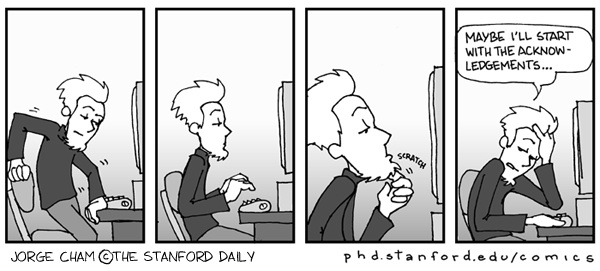
\includegraphics[width=\textwidth]{images/escrita.jpg}
		\fonte{http://www.phdcomics.com/comics/archive.php?comicid=149}
	\end{minipage}
\end{figure}

\subsection{Tabelas}
A Tabela~\ref{tab:estacoes} é um exemplo de tabela elaborada pelo(a) próprio(a) autor(a).

\begin{table}
	\caption{Período das estações do ano no Brasil}
	\label{tab:estacoes}
	\centering%
	\begin{minipage}{.6\textwidth}
		\begin{tabular*}{\textwidth}{ll}
			\hline
			\textbf{Meses} & \textbf{Estações do Ano}\\
			\hline
			21 de março a 21 de junho & Outono\\
			21 de junho a 23 de setembro & Inverno\\
			23 de setembro a 21 de dezembro & Primavera\\
			21 de dezembro a 21 de março & Verão\\
			\hline
		\end{tabular*}
		\fonte{Elaborada pela autora.}
	\end{minipage}
\end{table}

\section{Resumo}
O resumo deve conter de 100 a 500 palavras. No resumo não deve haver citações e indica-se que essa seja a última seção do texto a ser escrita. Veja abaixo uma sugestão de organização e exemplo de resumo de \cite{Moro11}.

Sugestão (uma a três linhas para cada item):
\begin{itemize}
	\item Contexto geral e específico;
	\item Questão/problema sendo investigado (propósito do trabalho);
	\item Estado-da-arte (por que precisa de uma solução nova/melhor);
	\item Solução (nome da proposta, metodologia básica sem detalhes, quais características respondem as questões iniciais, interpretação dos resultados, conclusões).
\end{itemize}


%=======================================================================
% Exemplos de Citações e Referências Bibliográficas
%=======================================================================
\chapter{Mais um capítulo}
Texto do capítulo.

\section{Nova seção}
Texto da nova seção. Segundo \citeonline{inproceedings}, esta é uma forma diferente de referenciar.

\subsection{Subseção}
Texto da subseção, com exemplo de citação \cite{book}.

\subsection{Subseção}
Texto da subseção, com exemplo de citação \cite{article}.

\section{Nova seção}
Texto da subseção, com exemplo de citação \cite{inproceedings}.

%=======================================================================
% Referências
%=======================================================================
\bibliography{exemplo}

%=======================================================================
% Exemplo de Apêndice
% O Apêndice é utilizado para apresentar material complementar elaborado
% pelo próprio autor.  Deve seguir as mesmas regras de formatação do
% corpo principal do documento.
%=======================================================================
\appendix
\chapter{Informações Complementares}

O Apêndice é o lugar para incluir textos complementares, que não são essenciais para o entendimento do assunto principal da monografia, mas que podem contribuir com informação relevante (por exemplo, uma prova matemática, uma conceituação básica, etc.).  Ele deve seguir o formato normal do documento.

%=======================================================================
% Exemplo de Anexo
% O Anexo é utilizado para a ``inclusão de materiais não elaborados pelo
% próprio autor, como cópias de artigos, manuais, folders, balancetes, etc.
% e não precisam estar em conformidade com o modelo''.
%=======================================================================
\annex
\chapter{Artigos Publicados}
Existe diferença entre os Apêndices e os Anexos.  Os apêndices trazem informação escrita pelo próprio autor do trabalho, incorporando-se ao formato da monografia como um todo.  Já um anexo é um material à parte, definido/publicado por si só, e que o autor julga conveniente ser apresentado juntamente com a monografia.  Normalmente também vai apresentar formato próprio, como um artigo publicado, um folder, uma planilha, etc.
\end{document}
